\subsection{Matched-time radial and angular error diagnostics}
\label{sec:review-profiles}

The maximum errors in the qualification tables need not occur at the same time, grid, or reference. We therefore reanalyse the hash-bound CPU controls corresponding to the qualified high-resolution RFM41 (seed 7331), Legendre36, and FD184 trajectories. The first two use the original $t_s=8$ schedule and retain the same nonzero-mode rank 40. The uniform RFM41 and Legendre36 controls are also included in the machine-readable results. Both existing FD448/$K=144$ references are reconstructed: \texttt{angular\_fine} uses rate 384 and \texttt{time\_fine} rate 512. No reference or candidate is integrated for this analysis. All 19 physical times are retained; the figures show the common times $8,24,48,72$ against \texttt{time\_fine}. There is no phase alignment.

Let $e_f$ be the velocity-vector or scalar-vorticity error and let $\langle\cdot\rangle_\theta$ denote the angular mean. For the existing layer144 radial nodes and physical-area weights $w_i$, define
\begin{equation}
R_f^2=\frac{\sum_i w_i\langle|f_{\rm ref}(r_i,\cdot)|^2\rangle_\theta}{\sum_i w_i},
 \qquad P_f(r_i)=\frac{\langle|e_f(r_i,\cdot)|^2\rangle_\theta^{1/2}}{R_f}.
\label{eq:review-profile-norm}
\end{equation}

This normalization avoids dividing by a locally vanishing field. For real fields represented by nonnegative Fourier modes, the angular error contribution is
\begin{equation}
Q_{f,k}=\left(\frac{c_k\sum_i w_i|\widehat e_{f,k}(r_i)|^2}
 {\sum_i w_i\langle|f_{\rm ref}(r_i,\cdot)|^2\rangle_\theta}\right)^{1/2},
 \qquad c_0=1,\quad c_k=2\;(k>0).
\label{eq:review-modal-error}
\end{equation}

For velocity, squared component magnitudes are summed in the polar representation $(u_r,u_\theta)$. The integrated vector-error energy is invariant under the pointwise orthogonal change to Cartesian components, but its allocation among angular modes depends on that representation; the displayed velocity spectrum is therefore a polar-component spectrum. Hence the weighted mean of $P_f^2$ and the sum of $Q_{f,k}^2$ both give the squared relative field error. The exact angular Parseval calculation agrees with the original layer144 physical-grid score to $2.13\times10^{-17}$ in 380 checks. Modes above the candidate cutoff $K=80$ contain the common unresolved reference tail, not additional candidate degrees of freedom.

\begin{figure}[htbp]
\centering
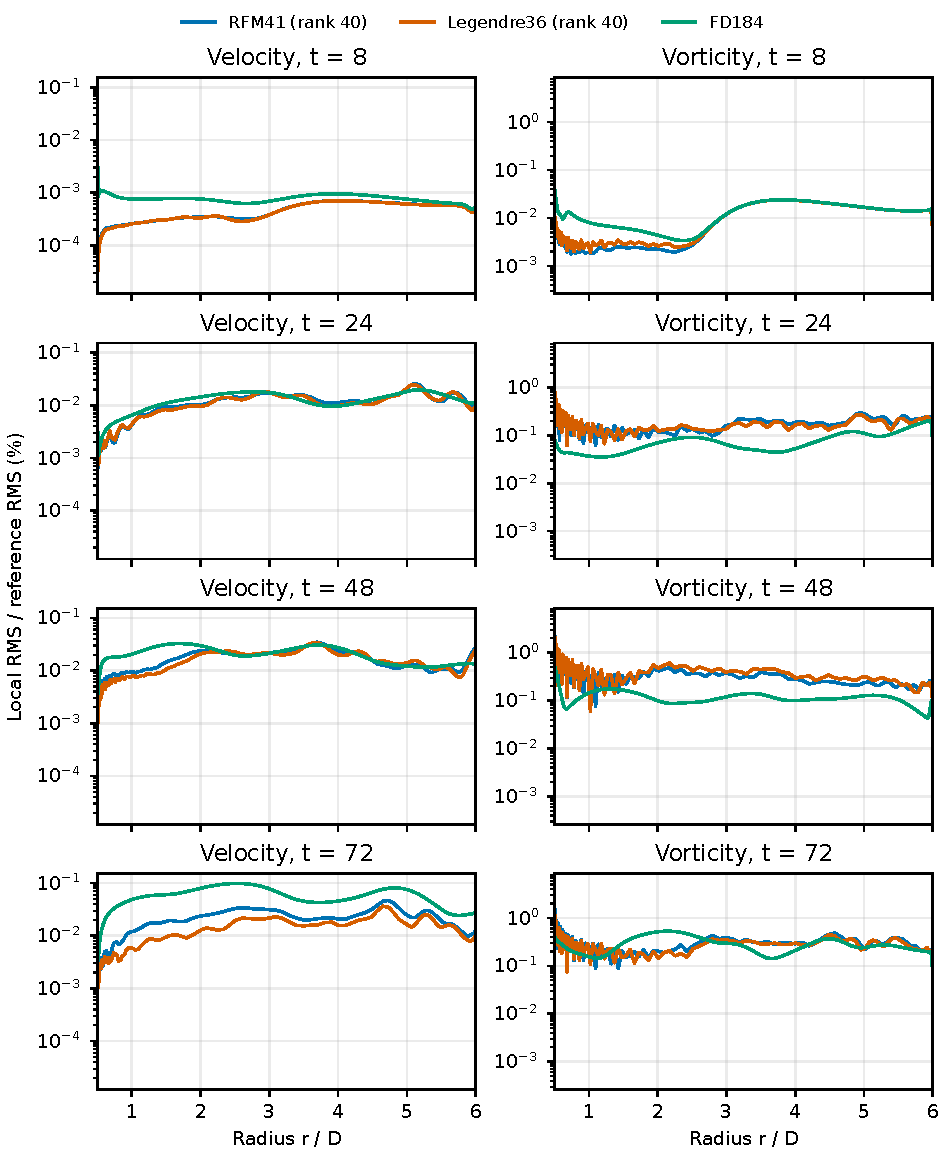
\includegraphics[width=\linewidth]{figures/review_radial_errors.pdf}
\caption{Matched-time radial error profiles $100P_f$ against the existing time-fine reference. RFM41 uses seed 7331. Galerkin curves use $t_s=8$; FD184 retains its qualified schedule. Curves share the same reference and times within each panel. The plotted quantity is a local angular RMS normalized by a global reference RMS, rather than a pointwise relative error.}
\label{fig:review-radial-errors}
\end{figure}

\begin{figure}[htbp]
\centering
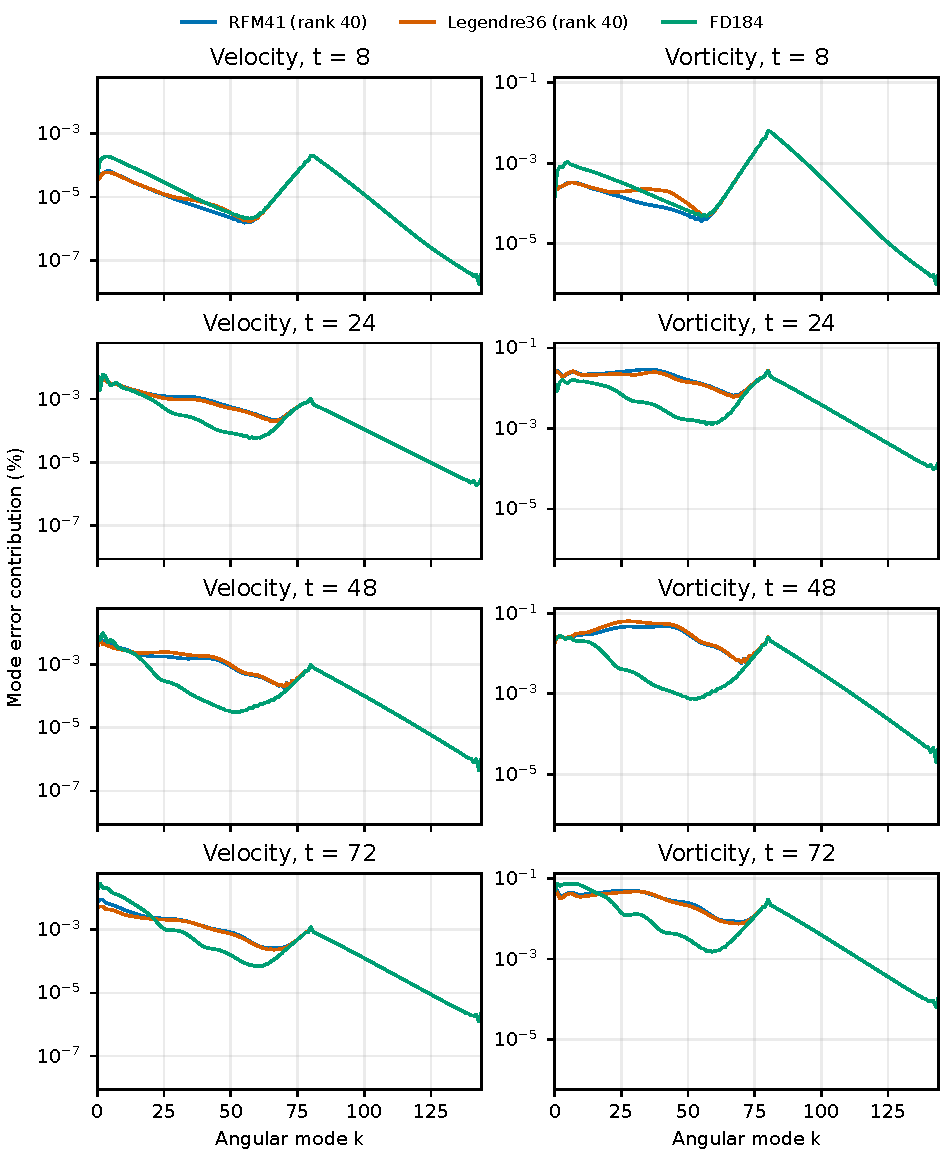
\includegraphics[width=\linewidth]{figures/review_angular_errors.pdf}
\caption{Angular error contributions $100Q_{f,k}$ for the same trajectories and times as Figure~\ref{fig:review-radial-errors}. Contributions combine in quadrature; they are not independently normalized modewise errors. The common tail above mode 80 reflects the finer reference spectrum.}
\label{fig:review-angular-errors}
\end{figure}

The original maxima are not a simultaneous ranking. For this RFM seed, the full-domain velocity and vorticity maxima occur at $t=72$ and $60$; the corresponding Legendre maxima occur at $60$ and $54$. In contrast, at the same $t=48$ and on layer144, RFM41, Legendre36, and FD184 have velocity errors $0.01886\%$, $0.01842\%$, and $0.02053\%$, but vorticity errors $0.29438\%$, $0.35509\%$, and $0.11317\%$. Thus even a simultaneous velocity ranking does not determine the vorticity ranking. Curl depends on first derivatives of velocity; an $L^2$ velocity comparison alone does not control their error. This observation is consistent with the measured spectra: at $t=72$, modes $k\le8$ contain $84.24\%$ of FD184's squared velocity-error norm, whereas modes $25\le k\le80$ contain $47.72\%$ of RFM41's squared vorticity-error norm, compared with $5.45\%$ for FD184.

The radial localization also requires qualification. At $t=72$, $61.14\%$ of RFM41's squared vorticity-error norm lies at $r\ge4$, but only $1.37\%$ lies at $r\ge5.9$. The observed error is therefore not confined to the narrow outermost layer. These diagnostics localize error in the full evolved solutions. They do not identify a causal benefit of the layer basis, or separate radial approximation, time discretization, boundary treatment, and reference uncertainty. The accompanying controlled ablation addresses basis attribution; the present figures alone do not.

\subsection{A CPU sensitivity experiment at $t_s=12$}
\label{sec:review-switch}

Revision 3 added four actual CPU trajectories through $T=72$: RFM37 and Legendre35 at rates $128\to112$, and RFM41 and Legendre36 at $152\to136$, switching at $t_s=12$ instead of 8. RFM uses seed 7331; the deterministic controls retain their original configurations. The generic CPU phase clock already accepts an explicit switch time. Its default observation list contains the old $t_s=8$ bridge instants, so this driver supplies the 19 common physical times explicitly. The underlying solver and archived data are unchanged. Four workers each use one BLAS thread; their elapsed times are not isolated performance evidence. Existing uniform and $t_s=8$ CPU controls are reused, rather than rerun or counted as new experiments.

All four new trajectories match the corresponding uniform CPU states exactly at the saved times $t\le12$. Both full-domain and near-field velocity and vorticity pass the $0.5\%$ threshold on all three grids against both frozen references; the per-cell triangle safeguard relative to the matching uniform control also passes, and alternating probe signs persist. Table~\ref{tab:review-switch12} reports full-domain field maxima separately from the worst safeguard across all four metrics. These are one-seed sensitivity results, not a new five-seed GPU qualification.

\begin{table}[htbp]
\centering\small
\begin{tabular}{llrrrr}
\hline
Configuration & Schedule & $E_u$ (\%) & $E_\omega$ (\%) & Guard (\%) & $N_{\rm nl}$\\
\hline
RFM37 & Uniform & 0.029428 & 0.409349 & 0.409349 & 9215\\
 & $t_s=8$ & 0.044672 & 0.431680 & 0.478647 & 8191\\
 & $t_s=12$ & 0.043821 & 0.429910 & 0.474465 & 8255\\
Legendre35 & Uniform & 0.026763 & 0.442065 & 0.442065 & 9215\\
 & $t_s=8$ & 0.041043 & 0.456649 & 0.497730 & 8191\\
 & $t_s=12$ & 0.040211 & 0.455435 & 0.493773 & 8255\\
RFM41 & Uniform & 0.018192 & 0.331380 & 0.331380 & 10943\\
 & $t_s=8$ & 0.025948 & 0.339890 & 0.368159 & 9919\\
 & $t_s=12$ & 0.025496 & 0.339258 & 0.365822 & 9983\\
Legendre36 & Uniform & 0.016132 & 0.362049 & 0.362049 & 10943\\
 & $t_s=8$ & 0.019717 & 0.366338 & 0.394046 & 9919\\
 & $t_s=12$ & 0.019410 & 0.365962 & 0.391767 & 9983\\
\hline
\end{tabular}
\caption{CPU switch-time sensitivity at the frozen spatial configurations. Errors maximize over two references, three grids, and 19 common times; each metric has its own argmax. The guard also includes the near-field metrics. RFM rows use seed 7331 and therefore need not equal the earlier five-seed maxima. $N_{\rm nl}$ counts actual nonlinear evaluations; the number of marching FFT batches is $2N_{\rm nl}$. No GPU trajectory is available for $t_s=12$, so no CPU--GPU bound is assigned to those rows.}
\label{tab:review-switch12}
\end{table}

Moving the switch from 8 to 12 adds 64 nonlinear evaluations and 128 FFT batches in every configuration. It removes 960 evaluations relative to the uniform schedules: $10.418\%$ at the middle scale and $8.773\%$ at the high scale, versus $11.112\%$ and $9.358\%$ for switching at 8. The measured error decrease is modest: for RFM37 the velocity maximum decreases by $0.000851$ percentage points and the vorticity maximum by $0.001771$ percentage points. The closest new safeguard is $0.493773\%$ for Legendre35. The later switch therefore trades a small increase in work for a small accuracy margin on this case; no isolated speed ranking follows.

The triggering transverse pulse terminates at $t=12$. Its $\sin^4$ profile is $C^3$ at that junction, with a possible fourth-derivative jump. The local Taylor consistency calculation for the bridge must respect the available one-sided regularity there. This experiment is a switch-time sensitivity test, not evidence that a smooth-transient order reduction has been removed. No timestep-refinement series is supplied to estimate an observed order. Separately, the archived $10^{-5}$ implementation gate compares CPU/GPU or CPU operator implementations of the \emph{same} discrete schedule. It is not a tolerance for changing from uniform to mixed timesteps; that change is assessed by the physical errors and the $0.5\%$ safeguard. In the quoted middle-scale RFM comparison, the velocity maxima $0.029428\%$ and $0.044672\%$ differ by $0.015244$ percentage points (about $51.8\%$ relatively), and both happen to occur at $t=72$. This relative increase alone establishes neither a transient-splitting mechanism nor order reduction.

\paragraph{A norm reduction is not a causal error budget.}
For the middle RFM velocity maxima, postponing the switch recovers approximately $5.584\%$ of the increase relative to the uniform schedule. This is the arithmetic ratio $(E_8-E_{12})/(E_8-E_U)$; it does not isolate a bridge-local error. The intervention simultaneously changes four time units of fine versus coarse integration, the bridge time and state, and the subsequent error history. Moreover, $t=8$ is inside the analytic pulse, not a nonsmooth forcing junction.

The saved fields make the nonadditivity explicit. Let $e_8=u_8-u_{\rm ref}$, $e_{12}=u_{12}-u_{\rm ref}$ and $\delta=e_8-e_{12}$, with a common physical-area inner product divided by $\|u_{\rm ref}\|^2$. Then
\begin{equation}
 \|e_8\|_{\rm ref}^2=\|e_{12}\|_{\rm ref}^2+
 2\langle e_{12},\delta\rangle_{\rm ref}+\|\delta\|_{\rm ref}^2.
 \label{eq:review-switch-attribution}
\end{equation}
At $t=72$ on layer144 against the time-fine reference, for RFM37 seed7331 these four terms are $1.9956194141\times10^{-7}$, $1.9202943907\times10^{-7}$, $7.4475738974\times10^{-9}$ and $8.4928450335\times10^{-11}$, respectively. They are squared relative errors, without percent scaling. The unrounded identity residual is $2.04\times10^{-22}$; the cross term accounts for about $98.87\%$ of the squared-norm difference. This deterministic identity illustrates why neither the $5.6\%$ recovery nor its $94.4\%$ complement is an independent physical error component. A causal bridge/coarse-step split would need separately controlled interventions and a timestep-refinement study.

